% !TeX encoding = UTF-8
% !TeX spellcheck = es_ES
% !TeX root = ../ComponentCatalog.tex
%!TEX root=../ComponentCatalog.tex

%XT60




\begin{table}[H]
    \centering
    \renewcommand\theadfont{\bfseries}
    \setlength{\tabcolsep}{10pt}
    \renewcommand{\arraystretch}{1.5}

    \begin{tabular}{|c|c|c|c|c|}
        \beginConnectorTable{Serie XT60}
        \connectorblockinfo{Fabricante}{China-Amass }
        \multirow{9}{*}{\makecell{Macho \\ Plug}}
        \connectordata{
            \begin{scope}
                \clip (0,0) rectangle  +(3,1.5);
                \node[inner sep=0pt, rotate=0] at (1.5,0.75)
                    {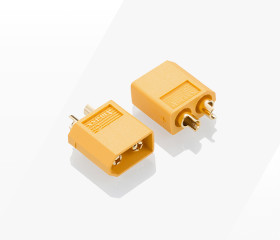
\includegraphics[scale=1.4]{pictures/connectors/XT60/XT60-M.jpg}};
            \end{scope}
        }{
            \pic[](pic) at(1.5,0.75){Xt60-M};
        }{TME}{XT60-M} {500V} {30A}
        %\cline{1 - 2}
        \connectorinfo{Codigo}{XT60-M}{\tabitem Para Cable}
        \connectordata{
            \begin{scope}
                \clip (0,0) rectangle  +(3,1.5);
                \node[inner sep=0pt, rotate=0] at (1.5,0.75)
                    {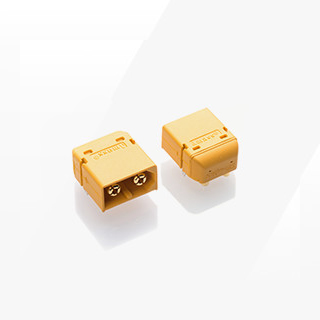
\includegraphics[scale=1.4]{pictures/connectors/XT60/XT60PW-M.jpg}};
            \end{scope}
        }{
            \pic[](pic) at(1.5,0.75){Xt60-M};
        }{TME}{XT60PW-M} {500V} {30A}
        \connectorinfo{Codigo}{XT60PW-M}{\tabitem Para PCB}
        
        \cline {1-2}

        \multirow{9}{*}{\makecell{Hembra \\ Socket}}
        \connectordata{
            \begin{scope}
                \clip (0,0) rectangle  +(3,1.5);
                \node[inner sep=0pt, rotate=0] at (1.5,0.75)
                    {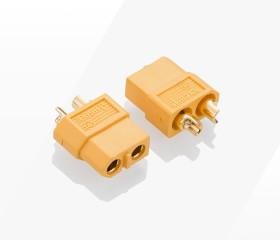
\includegraphics[scale=1.4]{pictures/connectors/XT60/XT60-F.jpg}};
            \end{scope}
        }{
            \pic[](pic) at(1.5,0.75){Xt60-F};
        }{TME}{XT60-F} {500V} {30A}
        %\cline{1 - 2}
        \connectorinfo{Codigo}{XT60-F}{\tabitem Para Cable}
        \connectordata{
            \begin{scope}
                \clip (0,0) rectangle  +(3,1.5);
                \node[inner sep=0pt, rotate=0] at (1.5,0.75)
                    {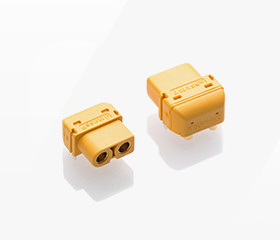
\includegraphics[scale=1.4]{pictures/connectors/XT60/XT60PW-F.jpg}};
            \end{scope}
        }{
            \pic[](pic) at(1.5,0.75){Xt60-F};
        }{TME}{XT60PW-F} {500V} {30A}
        \connectorinfo{Codigo}{XT60PW-F}{\tabitem Para PCB}
        
        \cline {1-2}

        \connectorblockinfo{Uso}{Paso Señal DCC}
        \connectorblockinfo{Ubicacion}{CJ}
        \noalign{\vskip 2mm}
        \beginConnectorTable{Serie XT60I}
        \connectorblockinfo{Fabricante}{China-Amass }
        \multirow{4}{*}{\makecell{Macho \\ Plug}}
        \connectordata{
            \begin{scope}
                \clip (0,0) rectangle  +(3,1.5);
                \node[inner sep=0pt, rotate=0] at (1.5,0.75)
                    {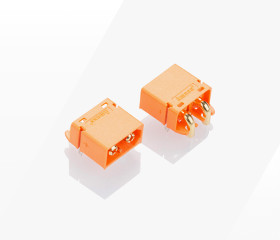
\includegraphics[scale=1.4]{pictures/connectors/XT60/XT60IPW-M.jpg}};
            \end{scope}
        }{
            \draw (0,0) rectangle (3,1.5) ;
        }{TME}{XT60IPW-M} {500V} {30A}
        \connectorinfo{Codigo}{XT60IPW-M}{\tabitem Para PCB}
        \cline{1 - 2}


        \multirow{4}{*}{\makecell{Hembra \\ Socket}}
        \connectordata{
            \begin{scope}
                \clip (0,0) rectangle  +(3,1.5);
                \node[inner sep=0pt, rotate=0] at (1.5,0.75)
                    {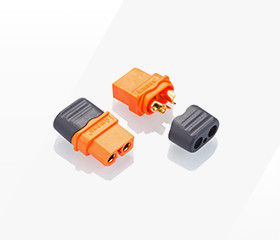
\includegraphics[scale=1.4]{pictures/connectors/XT60/XT60I-F.jpg}};
            \end{scope}
        }{
            \draw (0,0) rectangle (3,1.5) ;
        }{TME}{XT60I-F} {500V} {30A}
        \connectorinfo{Codigo}{XT60I-F}{\tabitem Para Cable}
        \cline{1 - 2}


        \connectorblockinfo{Uso}{Paso Señal DCC, con Deteccion}
        \connectorblockinfo{Ubicacion}{CJ}
    \end{tabular}
    \caption{Serie XT60}
    \label{tab:XT60}
\end{table}